\chapter{Quantum computing: from hardware to software}
\label{chapter2}

In this chapter, we briefly discuss how a quantum computer is realized. Today these computers are small, noisy, and not nearly as powerful as current classical computers, but Noisy Intermediate-Scale Quantum (NISQ) computers will be available in the next few years. Here “intermediate scale” refers to the size of quantum computers with a number of qubits ranging from 50 to a few hundred; that’s beyond what can be simulated by brute force using the most powerful existing classical supercomputers \cite{PreskillNote}.

In particular, we focus on the hardware and software of the quantum computers developed by the companies IBM and Google. We illustrate the 'superconducting qubits'  technology, on which both of the IBM and Google hardware are based upon. It is important to underline that this chapter is only a brief introduction to the quantum hardware and that a deep analysis is beyond the aim of this Thesis. 
 Then, we discuss about the software, needed as an interface between the quantum hardware apparatus and final users. In particular, the quantum software frameworks provided by IBM and Google are Qiskit and Cirq, respectively. This section gives tools to create a quantum circuit on each software, run them on a simulator or a real quantum device, when provided, and view the data results. Both software use Python programming language. 

%Decades of research at IBM has convinced us that superconducting qubits (versus other alternatives to building qubits) is the most controllable and scalable technology for the long term and the best path to achieving early quantum advantage. Our qubits are fabricated and packaged into quantum processors that are cooled within readily available cryogenic systems and controlled through customized room temperature microwave electronics.


\section{Quantum hardware: superconducting qubits}
The implementation of a real quantum hardware must satisfy five conditions, called DiVincenzo's criteria \cite{Divincenzo}:

\begin{enumerate}
	\item \textbf{Scalability}: a scalable physical system with well characterized qubits.
	\item \textbf{Reset}: the ability to initialize the state of the qubits to a simple fiducial state, such as $\ket{000\dots0}$.
	\item \textbf{Long decoherence times}: long relevant decoherence times, much longer than the gate operation time.	
	\item \textbf{'Universal' gate}: a `universal' set of quantum gates.
	\item \textbf{Efficiently read-out}: a qubit-specific measurement capability.
\end{enumerate}

One of the main challenges of implementing an efficient quantum hardware is to keep the system decoupled from external influences, except during the write, control and measurement phases \cite{Hardware} . One of the main approaches for implementing a quantum computer is based upon 'quantum integrated circuits', where qubits are constructed from collective electrodynamic modes of macroscopic electrical elements. The advantage is that qubits may be coupled together via non-dissipative linear electrical elements as capacitors, inductors and transmission lines. The difficult part is isolating these qubits from the external noise. 
The first requirement for an integrated circuit, in order to behave quantum mechanically, is the absence of dissipation for all metallic parts that constitute the circuit at the qubit operating temperature. 
Therefore, the low temperature superconductors are the best choice for this task and such a quantum integrated circuit implementation is called `\textit{superconducting qubit}'. The temperature of the integrated circuit has to be also less than the energy associated to the transition between the ground state, $\ket{0}$, and the excited state $\ket{1}$. The temperature of the wires of the control and read-out gates connected to the chip has to be low too. Quantum signal processing is performed in integrated circuit by non-linear dissipative elements that consist of superconducting tunnel junctions, also called Josephson junctions. 



\subsection{Josephson junctions}
The Josephson junctions are used in quantum integrated circuits because they are the only electronic elements that are both non-dissipative (in a good approximation) and non-linear at arbitrarily low temperature. 
They are constituted by two layers of superconducting films separated by a thin insulating layer, as illustrated in Figure \ref{junction}. The Josephson junctions are based on the tunnel effect: the insulating layer is thin enough to allow tunneling of discrete charges through the barrier \cite{Hardware2}. In fact, at low temperatures, the superconducting films produce \textit{Cooper's pairs} that can pass trough the potential wall, originating a charge flow.


\begin{figure}[h!]
\centering 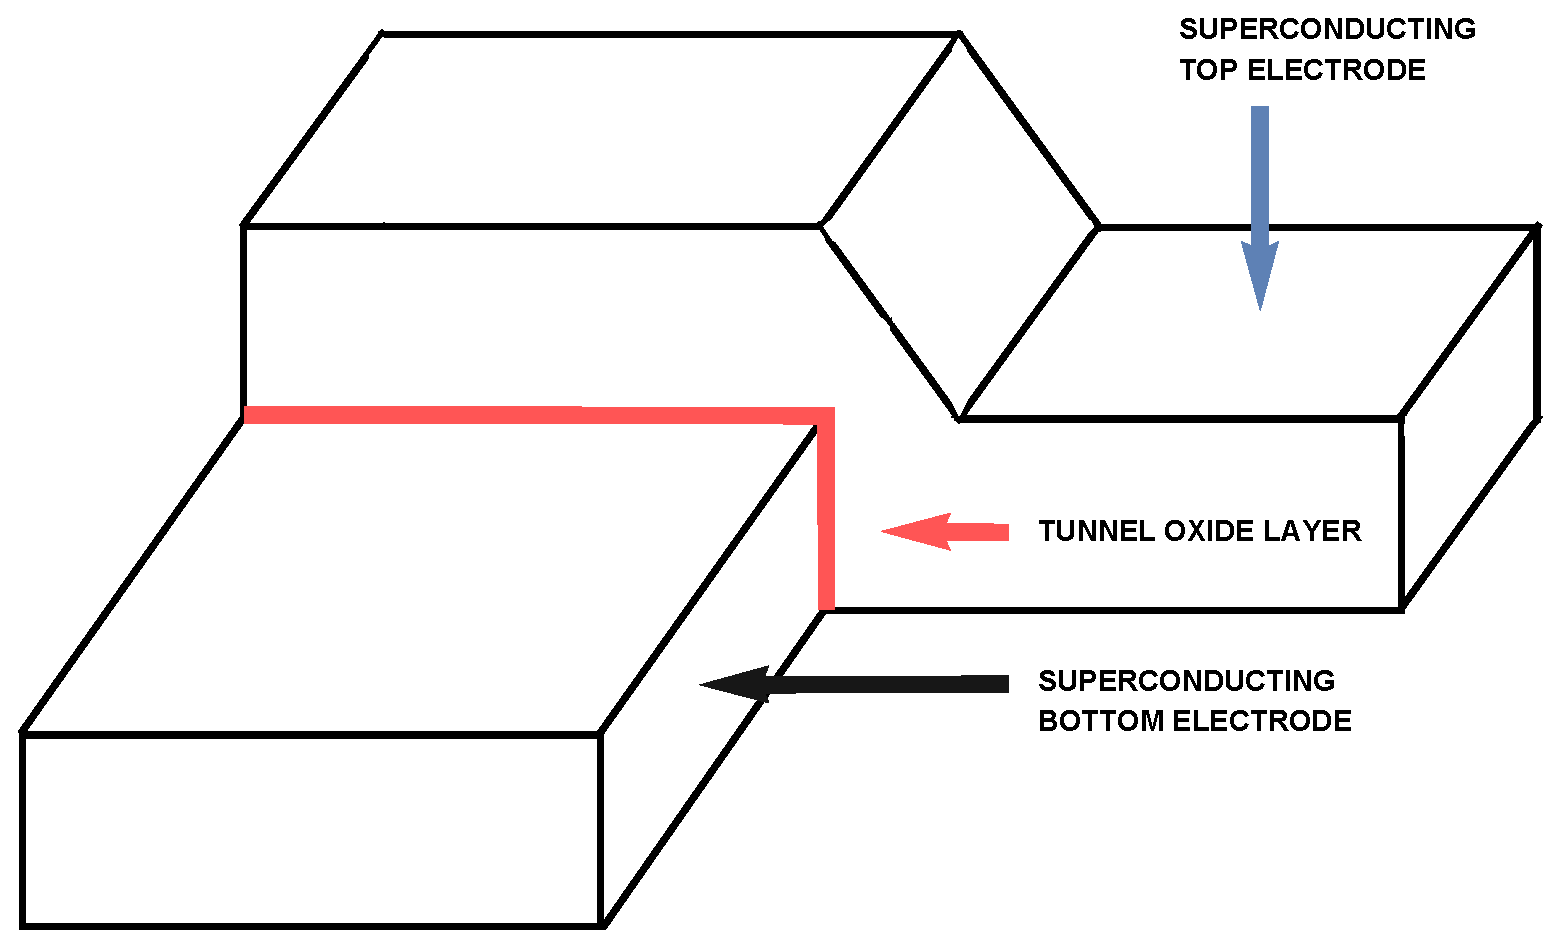
\includegraphics[width=0.4\textwidth]{./chapter2/image/junction.eps}
\caption{\label{junction} A Josephson junction realized with two superconducting thin films separated by an insulating layer that allow tunneling of discrete charges through the barrier.  }
\end{figure}

The most simple single qubit implementation using Josephson junctions is the charge qubit.
A 'charge qubit' is obtained by biasing the Josephson junction, that has an intrinsic capacity $C_J$, with a voltage source $U_g$ in series with a capacitor $C_G$, as shown in Figure \ref{CircuitJosephson}. The Cooper's pairs could not pass trough the capacitor shells without spending energy, therefore the superconducting layer exposed to the capacitor is called \textit{island}. The junction can be described by two parameters: $N_g$, the number of Cooper's pairs in the island, and $\theta$ that is called 'superconductive phase'. The Hamiltonian of such a system is:

\begin{equation}
H= E_C (N-N_g)^2 - E_J \cos{\theta} \qquad [\theta,N] = i
\end{equation}

\noindent where $E_C=\frac{ (2e)^2}{(2(C_J+C_g))}$ is the charging energy of the island of the box ($e$ represents the electron charge) and $E_J$ is called \textit{Josephson's energy}.

\tikzset{cross/.style={cross out, draw, 
         minimum size=2*(#1-\pgflinewidth), 
         inner sep=0pt, outer sep=0pt}}
\tikzset{component1/.style={draw,thick,circle,fill=white,minimum size =0.75cm,inner sep=0pt}}
\tikzset{component2/.style={draw,thick,rectangle,fill=white,minimum size =0.75cm,inner sep=0pt}}


\begin{figure}[h!]
\centering
% 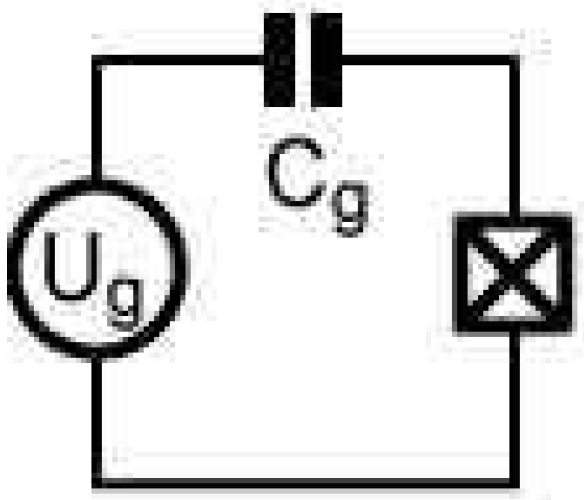
\includegraphics[width=0.15\textwidth]{./chapter2/image/junction_scheme.png}
\begin{circuitikz}[scale=0.6, transform shape]
\draw (0,0) to[esource] (0,4);
\node[fit={(0,0) (0,4)}, inner sep=0pt, label=center:U$_\mathrm{g}$] (0,2) {};
\draw (0,4) to[C, label=$C_g$] (4,4);
\node (S1) at (4,2) {};
\quadrato{S1}{0};
\draw (4,4) -- (4,2 + \sl);
\draw (4,2 - \sl) -- (4,0);
\draw (4,0) -- (0,0);
\end{circuitikz}

    \caption{\label{CircuitJosephson} Charge qubit circuit scheme. The $U_g$ represents a voltage source in series with a capacitor $C_G$, while the square box represents a Josephson junction.}
\end{figure}

\noindent The Hamiltonian could be wrote in the basis of the Cooper's pairs $\ket{N}$ as:

\begin{equation}
H = E_C \sum_N (N - N_g)^2 \ket{N}\bra{N} - \frac{1}{2} E_J \sum_N \ket{N+1}\bra{N} + \ket{N} \bra{N+1}
\label{HamiltonianCooper_N}
\end{equation}

\noindent where the second term is a coupling term, that relates the state $\ket{N}$ with the state $\ket{N+1}$.





\section{Quantum software: Qiskit and Cirq}
Today, a wide range of quantum computing software is available \cite{SoftwareComparisonGeneral}. Most of the quantum computing companies, as IBM, grant the access to a real quantum computer thanks to the cloud platform and the interaction between users and quantum computers is mediated by a software platform with API (Application Programming Interface) access \cite{SoftwareComparisonCirq}. Other companies, such as Google, have no current capability to connect to a quantum computer and provide just the simulator as yet.
Many practical considerations emerge when using a software interface to communicate with a real or simulated quantum computer. For example, we can ask how easy is to create, work with and manipulate quantum circuits or how easy is to parametrize algorithms for near-term quantum computing. Another good question can be asking quantum computer simulator can be used to test algorithms, how many qubits can be simulated and if the simulator is noiseless or noisy. If the platform gives access to real quantum devices, we can ask what are their main features, as the number of qubits or gate operations natively built-in. It's also important to understand how data results can be visualized.
 In this section we try to answer to these questions for the quantum software frameworks of IBM and Google, Qiskit and Cirq respectively. The first one provides the access to real quantum devices, the second one only makes simulators available.

\subsection{Qiskit software}
Qiskit is an open-source framework for working with the OpenQASM quantum language and quantum processors in the IBM Q experience \cite{DocumentationQiskit}.
It is organized in four distinct components:
\begin{itemize}
\item \textbf{Terra}: Qiskit Terra provides tools for composing quantum circuits at the level of quantum machine code and manages the execution of that code on quantum hardware. It also provides tools to 					allow quantum circuits to be optimized for a particular device.
\item \textbf{Aer}: Qiskit Aer provides simulators for studying quantum computing algorithms and applications in devices affected by noise; it permits to build noise models for noisy simulations.
\item \textbf{Ignis}: Qiskit Ignis includes tools for characterizing errors through method as tomography and for doing quantum error-correction.
\item \textbf{Aqua}: Qiskit Aqua provides quantum algorithms that can be directly used to build applications for quantum computing.
\end{itemize}


\subsubsection{Manipulating a quantum circuit}

Generally, a quantum circuit on Qiskit terra can be built in three main steps:
\begin{enumerate}
	\item Suppose $n$ and $m$ fixed integer. In general, a quantum circuit is composed by two registers: a quantum register of $n$ qubits and a classical register of $m$ bits.
	\item Each qubit of the quantum register has an initial state of $\ket{0}$. Quantum gates can be applied on the $n$ qubits available for changing the quantum state.
	\item The quantum circuit created can be visualized choosing the desired output.
\end{enumerate}
\vspace{0.2cm}
\noindent All the possible unitary gates can be implemented by defining a sequence of simpler gates implemented in the hardware. Then, there are options for doing measurement or reset of the state to $\ket{0}$, in the middle of the computation.

It is important to underline that the qubits of a multi-qubit system in Qiskit are ordered with the first qubit on the right-most side and the last qubit on the left-most side. Therefore, the gate matrix representation is different to the gate matrix form illustrated in the Chapter \ref{Chapter1}, but the difference is slightly so we don't illustrate the correct matrix form implemented in Qiskit.

An example of how to build and manipulate a quantum circuit is shown in Figure \ref{BuildCircuit_QFT}. Here, we do the quantum Fourier transform of the state $\ket{000}$, implementing the quantum Fourier transform (QFT) protocol for $n=3$ qubits \cite{Nielsen}.


\begin{figure}[h!]
\begin{lstlisting}[language=Python]%[language=Python, caption=Python example]

from qiskit import QuantumCircuit, ClassicalRegister, QuantumRegister
from math import pi
#select the number of qubit
n = 3 
#define the registers and create the quantum circuit
q = QuantumRegister(n,'q')  
c = ClassicalRegister(n,'c') 
circ = QuantumCircuit(q, c)
#add gate operation
circ.h(q[0])
circ.cu1(pi/2,q[1], q[0])
circ.cu1(pi/4,q[2], q[0])
circ.h(q[1])
circ.cu1(pi/2,q[2], q[1])
circ.h(q[2])
circ.swap(q[0],q[2])
for i in range(n):
    circ.measure(q[i], c[i])
#draw the circuit
circ.draw(output='latex')
 
\end{lstlisting}

\begin{equation*}
    \Qcircuit @C=1.0em @R=0.5em @!R {
	 	\lstick{q_{0}: \ket{0}} & \gate{H} & \control\qw & \dstick{\frac{\pi}{2}}\qw & \control\qw & \dstick{\frac{\pi}{4}}\qw & \qw & \qw & \qw & \qw & \qw & \qw & \qw & \qswap & \meter & \qw & \qw & \qw & \qw & \qw & \qw & \qw\\
	 	\lstick{q_{1}: \ket{0}} & \qw & \ctrl{-1} & \qw & \qw & \qw & \qw & \gate{H} & \control\qw & \dstick{\frac{\pi}{2}}\qw & \qw & \qw & \qw & \qw & \qw & \qw & \meter & \qw & \qw & \qw & \qw & \qw\\
	 	\lstick{q_{2}: \ket{0}} & \qw & \qw & \qw & \ctrl{-2} & \qw & \qw & \qw & \ctrl{-1} & \qw & \qw & \gate{H} & \qw & \qswap \qwx[-2] & \qw & \qw & \qw & \qw & \meter & \qw & \qw & \qw\\
	 	\lstick{c_{0}: 0} & \cw & \cw & \cw & \cw & \cw & \cw & \cw & \cw & \cw & \cw & \cw & \cw & \cw & \cw \cwx[-3] & \cw & \cw & \cw & \cw & \cw & \cw & \cw\\
	 	\lstick{c_{1}: 0} & \cw & \cw & \cw & \cw & \cw & \cw & \cw & \cw & \cw & \cw & \cw & \cw & \cw & \cw & \cw & \cw \cwx[-3] & \cw & \cw & \cw & \cw & \cw\\
	 	\lstick{c_{2}: 0} & \cw & \cw & \cw & \cw & \cw & \cw & \cw & \cw & \cw & \cw & \cw & \cw & \cw & \cw & \cw & \cw & \cw & \cw \cwx[-3] & \cw & \cw & \cw\\
	 }
\end{equation*}
\caption{\label{BuildCircuit_QFT} Top: the source python code in Qiskit for building the quantum circuit of QFT algorithm for $n=3$ qubit is displayed. The QFT of the state $\ket{000}$ is done. Bottom: that quantum circuit is visualized in 'latex' output. The first three lines represent the quantum register, while the other three represent the classical register. }
\end{figure}



\subsubsection{Parameterized circuits}
Parameterization is a common feature of many quantum algorithms. Parameters/angles of an algorithm can be iteratively changed to minimize an energy or cost function.
A `Parameter' class is available and it can be used to specify a placeholder wherever a numeric parameter can be used.
For instance, we illustrate a single-qubit parameterized circuit in Figure \ref{ParameterizedCircuit_example}.

\begin{figure}[h!]

\begin{lstlisting}[language=Python]%[language=Python, caption=Python example]

from qiskit import QuantumCircuit, ClassicalRegister, QuantumRegister
from math import pi
from qiskit.circuit import Parameter
#define parameter k
k = Parameter('k')
#create the circuit
n = 1
circ = QuantumCircuit(1, 1)
circ.rz(k, range(1))
 
\end{lstlisting}

\caption{\label{ParameterizedCircuit_example} Example of a parameterized circuit for $n=1$ qubit in Qiskit software.}
\end{figure}

\newpage
\subsubsection{Running a quantum circuit}

First of all, let us focus on what 'running a quantum circuit' actually means. In a given run of a quantum circuit with $n$ measurements, the result will be one of the $2^n$ possible n-bit binary strings. If the experiment is run for a second time, even if the measurement is perfect and has no error, the outcome may be different, due to the fundamental randomness of quantum physics. The results of a quantum circuit executed many different times can be represented as a distribution over the full $2^n$ possible outcomes. It is not scalable to represent all possible outcomes; therefore, we keep only those outcomes that happen in a given experiment, and represent them as a histogram. In the histogram/bar graph representation the height of the bar represents the fraction of instances the outcome occurs during the experiment. Only those outcomes that occurred at least once are included. If all the bars are too small for visualization, they are collected into single bar called “other values”. 

Qiskit provides a useful interface for running quantum circuits. It is composed by three main components: the providers, which access backends and provide backend object, the backends, that run the quantum circuit, and the jobs, that keep track of the submitted jobs on a real hardware.  There are two main providers available. The first one is the 'Qiskit Aer Provider' that includes backends to simulate the run of a quantum circuit on a quantum device. That simulation is done in a classical computer so exponential computational resources are used. The second provider is the 'IBM Q Provider' that support the access to IBM Quantum experience backends. 
Therefore, backends represent either a simulator or a real quantum computer and are responsible for running quantum circuits and returning results. 

\subsubsection{Simulators}

The simulators available to simulate a run of a quantum circuit on a quantum device are contained mainly in the Qiskit Aer provider. It includes three simulator backends:

\begin{itemize}
	\item {\fontfamily{lmtt}\selectfont qasm$\_$simulator}: is designed to mimic an actual device; allows ideal and noisy multi-shot executions of qiskit circuits and returns a count dictionary containing the final values of any classical register in the circuit.  The maximum number of qubits supported by this simulator is 28 qubits.
	\item {\fontfamily{lmtt}\selectfont statevector$\_$simulator}: allows ideal single-shot executions of qiskit circuits and returns the final statevector of the simulation. If a circuit contains measure or reset gate operations the 	final statevector will be a conditional statevector after simulating wave-function collapse to the outcome of a measure or reset. Also for this simulator the maximum number supported is of 28 qubits.
	\item {\fontfamily{lmtt}\selectfont unitary$\_$simulator}: allows ideal single-shot executions of qiskit circuits and returns the final unitary matrix of the circuit itself. Note that the circuit cannot contain measure or reset operations 		for this backend and the maximum number of qubits supported is 14 qubits.
\end{itemize}
\vspace{0.2cm}
\noindent The IBM Q Provider supports the access to IBM Quantum experience backends that contains a remote optimized simulator backend called  '{\fontfamily{lmtt}\selectfont ibmq$\_$qasm$\_$simulator}'. This remote simulator is accessible by a cloud service and is capable of simulating up to 32 qubits.

If none is specified the simulators are noiseless, otherwise it is possible to implement a noise model for doing noisy simulations. There are three key classes in Qiskit Aer for building a noise model: the 'NoiseModel' class which stores a noise model, the 'QuantumError' class which describes gate errors and the 'ReadoutError' which describes classical readout errors.


An example of how Qasm Simulator acts is shown in Figure \ref{QFT_qasm_melbourne}. In that example, the quantum circuit previously built as an instance, illustrated in Figure \ref{BuildCircuit_QFT}, is simulated on that backend. The results, that are plotted in the histogram on the left, are consistent with the theory \cite{Nielsen}, as expected in a noiseless simulation.




\subsubsection{Real quantum devices}
The IBM Quantum experience backends supported by IBM Q Provider are constituted by the remote simulator previously presented and by three real public quantum devices. They are made available publicly by IBM through a cloud service. 

\noindent Let us illustrate the real quantum device provided by IBM:

\begin{itemize}
	\item {\fontfamily{lmtt}\selectfont ibmq$\_$16$\_$melbourne}: the IBM Q Melbourne is a $n=14$ qubit real quantum device. 
	\item {\fontfamily{lmtt}\selectfont ibmqx2}: the IBM Q Yorktown ('ibmqx2') is a $n=5$ qubits real quantum device. 
	\item {\fontfamily{lmtt}\selectfont ibmqx4}: the IBM Q Tenerife ('ibmqx4') is a $n=5$ qubits real quantum device. 

\end{itemize}

\noindent For each device, the native gate implemented are $u_1$, $u_2$, $u_3$, $CX$, $\mathbb{I}$, whose matrix forms are illustrated in Chapter \ref{Chapter1}. For the IBM Q Melbourne, the device layout and its connectivity are shown in Figure \ref{MelbourneLayout}, while the Table \ref{ibmq_16_mealburne_parameters} shows experimental parameters for each qubit of this device. For the IBM Q Yorktown and 
IBM Q Tenerife, look at the Figure \ref{IBMQX2_X4_Layout} and the Table \ref{IBMQX2_X4_parameters}.

For instance, in Figure \ref{QFT_qasm_melbourne}, we execute the QFT circuit, previously illustrated in Figure \ref{BuildCircuit_QFT}, in the IBM Q Melbourne device. The histogram on the right shows the results obtained. They are very different from the one obtained by the ideal simulation, due to noise that affects the real hardware.

\vspace{0.1cm}
%%%%FIGURA LAYOUT IBMQ MELBOURNE%%%%
\begin{center}
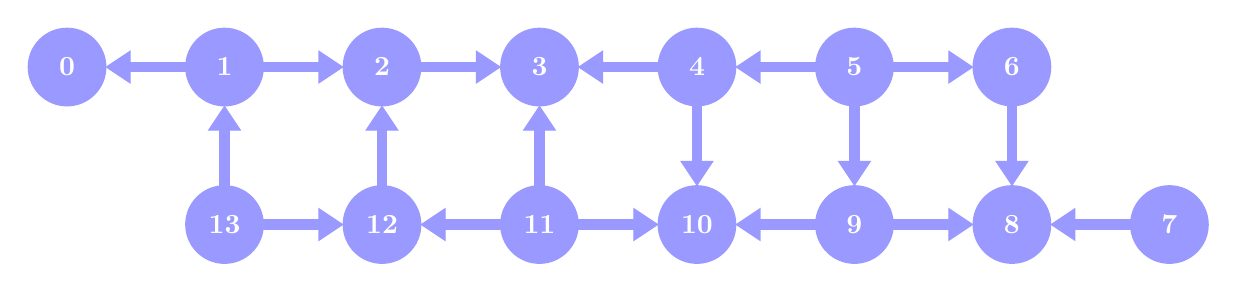
\begin{tikzpicture} %[scale=0.7, transform shape]

\draw[line width=1.3mm, color=blue!40!white] (0.8,0) -- (2,0); \filldraw[color=blue!40!white] (0.5,0) -- (0.8,0.2) -- (0.8,-0.2) -- (0.5,0); %freccia
\draw[line width=1.3mm, color=blue!40!white]  (2,0) -- (4-0.8,0); \filldraw[color=blue!40!white] (3.5,0) -- (3.2,0.2) -- (3.2,-0.2) -- (3.5,0); %freccia
\draw[line width=1.3mm, color=blue!40!white] (4,0) -- (6-0.8,0); \filldraw[color=blue!40!white] (5.5,0) -- (5.2,0.2) -- (5.2,-0.2) -- (5.5,0); %freccia
\draw[line width=1.3mm, color=blue!40!white]  (6+0.8,0) -- (8,0); \filldraw[color=blue!40!white] (6.5,0) -- (6.8,0.2) -- (6.8,-0.2) -- (6.5,0); %freccia
\draw[line width=1.3mm, color=blue!40!white]  (8+0.8,0) -- (10,0); \filldraw[color=blue!40!white] (8.5,0) -- (8.8,0.2) -- (8.8,-0.2) -- (8.5,0); %freccia
\draw[line width=1.3mm, color=blue!40!white]  (10,0) -- (12-0.8,0);  \filldraw[color=blue!40!white] (11.5,0) -- (11.2,0.2) -- (11.2,-0.2) -- (11.5,0); %freccia

\draw[line width=1.3mm, color=blue!40!white]  (2,0-0.8) -- (2,-2);  \filldraw[color=blue!40!white] (2,-0.5) -- (2.2,-0.8) -- (1.8,-0.8) -- (2,-0.5); %freccia
\draw[line width=1.3mm, color=blue!40!white]  (4,0-0.8) -- (4,-2); \filldraw[color=blue!40!white] (4,-0.5) -- (4.2,-0.8) -- (3.8,-0.8) -- (4,-0.5); %freccia
\draw[line width=1.3mm, color=blue!40!white]  (6,0-0.8) -- (6,-2); \filldraw[color=blue!40!white] (6,-0.5) -- (6.2,-0.8) -- (5.8,-0.8) -- (6,-0.5); %freccia
\draw[line width=1.3mm, color=blue!40!white]  (8,0) -- (8,-2+0.8); \filldraw[color=blue!40!white] (8,-1.5) -- (8.2,-1.2) -- (7.8,-1.2) -- (8,-1.5); %freccia
\draw[line width=1.3mm, color=blue!40!white]  (10,0) -- (10,-2+0.8); \filldraw[color=blue!40!white] (10,-1.5) -- (10.2,-1.2) -- (9.8,-1.2) -- (10,-1.5); %freccia
\draw[line width=1.3mm, color=blue!40!white]  (12,0) -- (12,-2+0.8); \filldraw[color=blue!40!white] (12,-1.5) -- (12.2,-1.2) -- (11.8,-1.2) -- (12,-1.5); %freccia


\draw[line width=1.3mm, color=blue!40!white]  (2,-2) -- (4-0.8,-2); \filldraw[color=blue!40!white] (3.5,-2) -- (3.2,0.2-2) -- (3.2,-0.2-2) -- (3.5,-2); %freccia
\draw[line width=1.3mm, color=blue!40!white]  (4+0.8,-2) -- (6,-2); \filldraw[color=blue!40!white] (4.5,-2) -- (4.8,0.2-2) -- (4.8,-0.2-2) -- (4.5,-2); %freccia
\draw[line width=1.3mm, color=blue!40!white]  (6,-2) -- (8-0.8,-2); \filldraw[color=blue!40!white] (7.5,-2) -- (7.2,0.2-2) -- (7.2,-0.2-2) -- (7.5,-2); %freccia
\draw[line width=1.3mm, color=blue!40!white]  (8+0.8,-2) -- (10,-2); \filldraw[color=blue!40!white] (8.5,-2) -- (8.8,0.2-2) -- (8.8,-0.2-2) -- (8.5,-2); %freccia
\draw[line width=1.3mm, color=blue!40!white]  (10,-2) -- (12-0.8,-2); \filldraw[color=blue!40!white] (11.5,-2) -- (11.2,0.2-2) -- (11.2,-0.2-2) -- (11.5,-2); %freccia
\draw[line width=1.3mm, color=blue!40!white]  (12+0.8,-2) -- (14,-2);  \filldraw[color=blue!40!white] (12.5,-2) -- (12.8,0.2-2) -- (12.8,-0.2-2) -- (12.5,-2); %freccia

\fill[fill=blue!40!white] (0,0) circle (0.5cm);
\fill[fill=blue!40!white] (2,0) circle (0.5cm);
\fill[fill=blue!40!white] (4,0) circle (0.5cm);
\fill[fill=blue!40!white] (6,0) circle (0.5cm);
\fill[fill=blue!40!white] (8,0) circle (0.5cm);
\fill[fill=blue!40!white] (10,0) circle (0.5cm);
\fill[fill=blue!40!white] (12,0) circle (0.5cm);


\fill[fill=blue!40!white] (2,-2) circle (0.5cm);
\fill[fill=blue!40!white] (4,-2) circle (0.5cm);
\fill[fill=blue!40!white] (6,-2) circle (0.5cm);
\fill[fill=blue!40!white] (8,-2) circle (0.5cm);
\fill[fill=blue!40!white] (10,-2) circle (0.5cm);
\fill[fill=blue!40!white] (12,-2) circle (0.5cm);
\fill[fill=blue!40!white] (14,-2) circle (0.5cm);


\node[text=white] at (0,0) {\textbf{0}};
\node[text=white] at (2,0) {\textbf{1}};
\node[text=white] at (4,0) {\textbf{2}};
\node[text=white] at (6,0) {\textbf{3}};
\node[text=white] at (8,0) {\textbf{4}};
\node[text=white] at (10,0) {\textbf{5}};
\node[text=white] at (12,0) {\textbf{6}};


\node[text=white] at (2,-2) {\textbf{13}};
\node[text=white] at (4,-2) {\textbf{12}};
\node[text=white] at (6,-2) {\textbf{11}};
\node[text=white] at (8,-2) {\textbf{10}};
\node[text=white] at (10,-2) {\textbf{9}};
\node[text=white] at (12,-2) {\textbf{8}};
\node[text=white] at (14,-2) {\textbf{7}};



\end{tikzpicture}
\captionof{figure}{Layout and connectivity on 'ibmq melbourne'. The arrows represent the coupling map of this device. }
\label{MelbourneLayout}
\end{center}
%%%%%%%%%%%%%%%%%%%%


\begin{figure}[h!]
\begin{minipage}[c]{0.5\linewidth}
\hspace{1cm}
\centering 
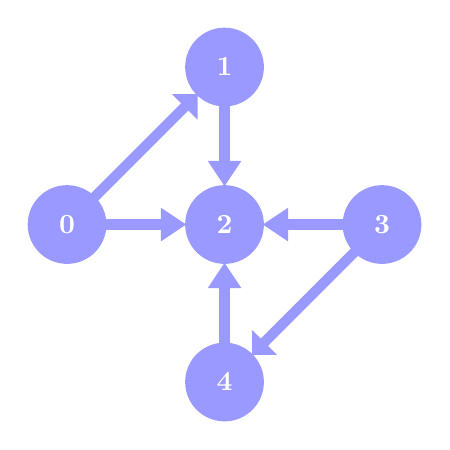
\begin{tikzpicture} %[scale=0.7, transform shape] %%Layout ibmx2


\draw[line width=1.3mm, color=blue!40!white]  (0,0) -- (2-0.8,0); \filldraw[color=blue!40!white] (1.5,0) -- (1.2,0.2) -- (1.2,-0.2) -- (1.5,0); %freccia
\draw[line width=1.3mm, color=blue!40!white]  (2+0.8,0) -- (4,0); \filldraw[color=blue!40!white] (2.5,0) -- (2.8,0.2) -- (2.8,-0.2) -- (2.5,0); %freccia

\draw[line width=1.3mm, color=blue!40!white]  (2,2) -- (2,0.8); \filldraw[color=blue!40!white] (2,0.5) -- (2.2,0.8) -- (1.8,0.8) -- (2,0.5); %freccia
\draw[line width=1.3mm, color=blue!40!white]  (2, -0.8) -- (2,-2); \filldraw[color=blue!40!white] (2,-0.5) -- (2.2,-0.8) -- (1.8,-0.8) -- (2,-0.5); %freccia

\draw[line width=1.3mm, color=blue!40!white]  (0,0) -- (2-0.45,2-0.45); \filldraw[color=blue!40!white] (1.65,1.65) -- (1.65,1.35) -- (1.35,1.65) -- (1.65,1.65); %freccia
\draw[line width=1.3mm, color=blue!40!white]  (2+0.45, -2+0.45) -- (4,0); \filldraw[color=blue!40!white] (2.35,-1.65) -- (2.65,-1.65) -- (2.65,-1.65) -- (2.35,-1.35); %freccia

\fill[fill=blue!40!white] (0,0) circle (0.5cm); 
\fill[fill=blue!40!white] (2,0) circle (0.5cm);
\fill[fill=blue!40!white] (4,0) circle (0.5cm);
\fill[fill=blue!40!white] (2,2) circle (0.5cm);
\fill[fill=blue!40!white] (2,-2) circle (0.5cm);

\node[text=white] at (0,0) {\textbf{0}};
\node[text=white] at (2,0) {\textbf{2}};
\node[text=white] at (4,0) {\textbf{3}};
\node[text=white] at (2,2) {\textbf{1}};
\node[text=white] at (2,-2) {\textbf{4}};

\end{tikzpicture}

\end{minipage}
\hspace{-1cm}
% \begin{large} $\Rightarrow$ \end{large}
\begin{minipage}[]{0.5\linewidth}
\centering 

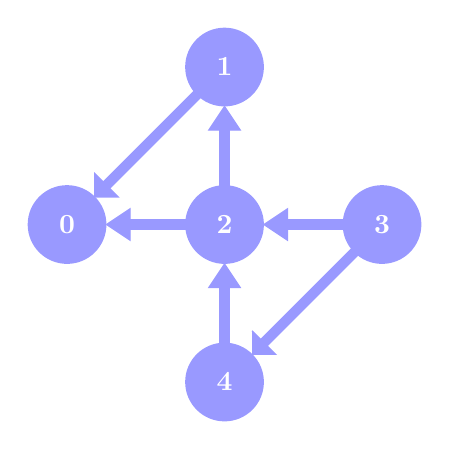
\begin{tikzpicture} %[scale=0.7, transform shape]  %%Layout ibmx4


\draw[line width=1.3mm, color=blue!40!white]  (0+0.8,0) -- (2,0); \filldraw[color=blue!40!white] (0.5,0) -- (0.8,0.2) -- (0.8,-0.2) -- (0.5,0); %freccia
\draw[line width=1.3mm, color=blue!40!white]  (2+0.8,0) -- (4,0); \filldraw[color=blue!40!white] (2.5,0) -- (2.8,0.2) -- (2.8,-0.2) -- (2.5,0); %freccia

\draw[line width=1.3mm, color=blue!40!white]  (2,2-0.8) -- (2,0); \filldraw[color=blue!40!white] (2,1.5) -- (2.2,1.2) -- (1.8,1.2) -- (2,1.5); %freccia
\draw[line width=1.3mm, color=blue!40!white]  (2, -0.8) -- (2,-2); \filldraw[color=blue!40!white] (2,-0.5) -- (2.2,-0.8) -- (1.8,-0.8) -- (2,-0.5); %freccia

\draw[line width=1.3mm, color=blue!40!white]  (0+0.45,0+0.45) -- (2,2); \filldraw[color=blue!40!white] (0.35,0.35) -- (0.65,0.35) -- (0.35,0.65) -- (0.35,0.35); %freccia
\draw[line width=1.3mm, color=blue!40!white]  (2+0.45, -2+0.45) -- (4,0); \filldraw[color=blue!40!white] (2.35,-1.65) -- (2.65,-1.65) -- (2.65,-1.65) -- (2.35,-1.35); %freccia

\fill[fill=blue!40!white] (0,0) circle (0.5cm); 
\fill[fill=blue!40!white] (2,0) circle (0.5cm);
\fill[fill=blue!40!white] (4,0) circle (0.5cm);
\fill[fill=blue!40!white] (2,2) circle (0.5cm);
\fill[fill=blue!40!white] (2,-2) circle (0.5cm);

\node[text=white] at (0,0) {\textbf{0}};
\node[text=white] at (2,0) {\textbf{2}};
\node[text=white] at (4,0) {\textbf{3}};
\node[text=white] at (2,2) {\textbf{1}};
\node[text=white] at (2,-2) {\textbf{4}};

\end{tikzpicture}

\end{minipage}
\caption{\label{IBMQX2_X4_Layout} Layout and connectivity on left of 'ibmqx2' and on right of 'ibmqx4'. The arrows represent the coupling map of these devices.}
\end{figure}




\begin{center}
\begin{table}[h!]
\[
\begin{array}{*{5}c}
\toprule
\text{Qubit} 	&	\text{Frequency (GHz)}	&	T_1 ( \mu s)	&	T_2 ( \mu s)	&	\text{Readout error}	\\
\midrule
Q_0	&	5.10	&	66.96	&	21.76	&	0.061 \\
Q_1	&	5.24	&	64.06	&	101.46	&	0.069 \\
Q_2	&	5.03	&	35.55	&	59.15	&	0.085 \\
Q_3	&	4.89	&	21.92	&	28.49	&	0.128 \\
Q_4	&	5.03	&	42.14	&	18.81	&	0.062 \\
Q_5	&	5.07	&	26.42	&	48.51	&	0.073 \\
Q_6	&	4.92	&	90.90	&	86.00	&	0.067 \\
Q_7	&	4.97	&	51.10	&	86.05	&	0.091 \\
Q_8	&	4.74	&	59.44	&	90.43	&	0.050 \\
Q_9	&	4.96	&	50.33	&	86.21	&	0.045 \\
Q_{10}	&	4.95	&	48.88	&	57.08	&	0.044 \\
Q_{11}	&	5.00	&	54.33	&	91.86	&	0.036 \\
Q_{12}	&	4.76	&	58.29	&	89.07	&	0.076 \\
Q_{13}	&	4.97	&	21.71	&	35.82	&	0.056 \\
\bottomrule

\end{array}
\]
\caption{Typical qubit parameters for the 'ibmq melbourne' device, where $T_1$ and $T_2$ are the relaxation times of the qubit. }
\label{ibmq_16_mealburne_parameters}
\end{table}
\end{center}














\begin{center}
\begin{table}[h!]
\[
\begin{array}{*{5}c}
\toprule
\text{Qubit} 	&	\text{Frequency (GHz)}	&	T_1 ( \mu s)	&	T_2 ( \mu s)	&	\text{Readout error}	\\
\midrule
Q_0	&	5.29	&	56.01	&	60.43	&	0.028 \\
Q_1	&	5.24	&	65.03	&	48.00	&	0.024 \\
Q_2	&	5.03	&	71.12	&	60.17	&	0.014 \\
Q_3	&	5.30	&	66.55	&	34.31	&	0.041 \\
Q_4	&	5.08	&	56.09	&	28.91	&	0.027 \\
\bottomrule

\end{array}
\]
\[
\begin{array}{*{5}c}
\toprule
\text{Qubit} 	&	\text{Frequency (GHz)}	&	T_1 ( \mu s)	&	T_2 ( \mu s)	&	\text{Readout error}	\\
\midrule
Q_0	&	5.25	&	38.64	&	14.22	&	0.059 \\
Q_1	&	5.30	&	52.83	&	9.97	&	0.079 \\
Q_2	&	5.34	&	47.49	&	29.52	&	0.182 \\
Q_3	&	5.43	&	48.66	&	27.64	&	0.356\\
Q_4	&	5.17	&	46.85	&	5.30	&	0.250 \\
\bottomrule

\end{array}
\]

\caption{Top: typical qubit parameters for the 'ibmqx2' device. Bottom: typical qubit parameters for the 'ibmqx4' device. $T_1$ and $T_2$ are the relaxation times of the qubit. }
\label{IBMQX2_X4_parameters}
\end{table}
\end{center}










\begin{figure}[h!]
\begin{lstlisting}[language=Python]%[language=Python, caption=Python example]

from qiskit import Aer, execute
from qiskit.tools.visualization import plot_histogram
# Select the QasmSimulator from the Aer provider
simulator = Aer.get_backend('qasm_simulator')
# Execute and get counts
result = execute(circ, simulator).result()
counts = result.get_counts(circ)
plot_histogram(counts, title='QFT algorithm counts')

from qiskit import *
IBMQ.load_accounts(hub=None)
from qiskit.tools.monitor import job_monitor, backend_monitor, backend_overview
# Select the IBM Q Melbourne backend
backend=IBMQ.get_backend('ibmq_16_melbourne')
# Execute and get counts
job = execute(circ,backend)
job_monitor(job)
result = job.result()
counts = result.get_counts(circ)
plot_histogram(counts, title='QFT algorithm counts')
 
\end{lstlisting}
\centering
\begin{minipage}[c]{0.5\linewidth}
\hspace{1cm}
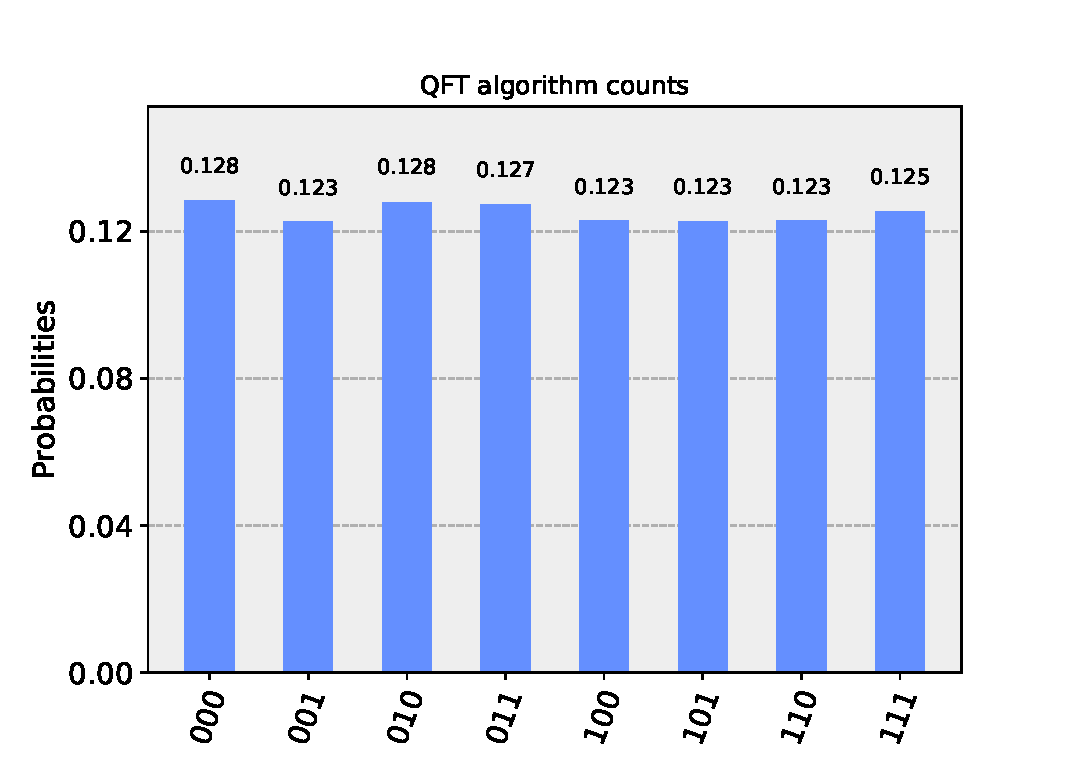
\includegraphics[width=0.75\textwidth]{./chapter2/image/QFT_qasm_simulator.eps} 
\end{minipage}
\hspace{-1cm}
% \begin{large} $\Rightarrow$ \end{large}
\begin{minipage}[]{0.5\linewidth}
\centering 
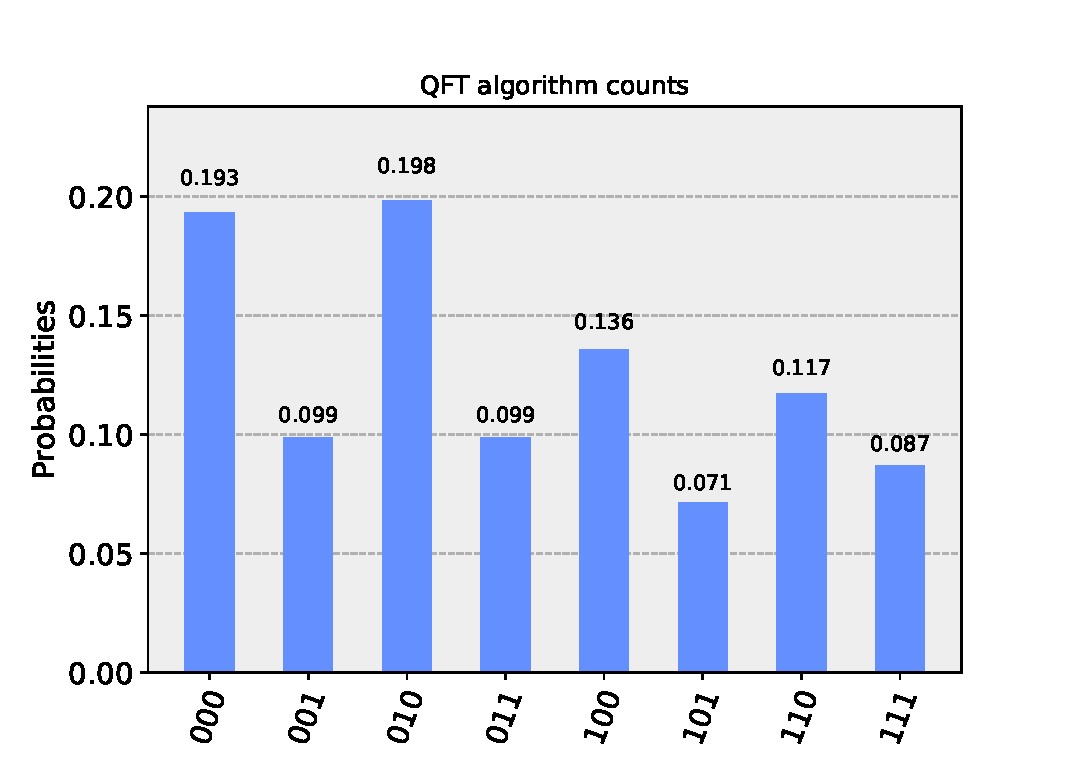
\includegraphics[width=0.75\textwidth]{./chapter2/image/QFT_ibmq_16_melbourne.eps} 
\end{minipage}
\caption{\label{QFT_qasm_melbourne} The QFT circuit described in Figure \ref{BuildCircuit_QFT} is executed both on Qasm Simulator, in ideal condition, and on IBM Q Melbourne. At the top the python code is reported and at the bottom the histograms of count results are displayed. 
Left histogram: Qasm Simulator counts. The results are very closed to the one expected by the theory.
Right histogram: IBM Q Melbourne counts. The results are different from the one obtained in the ideal case, due to the noise that affects the real hardware.}

\end{figure}




\subsection{Cirq software}
 \label{Cirq_section}
Cirq is an open-source framework for editing Noisy Intermediate Scale Quantum (NISQ) circuits. It provides a python library for working with quantum circuits and a high-performance local quantum circuit simulator.
Cirq is still under development \cite{DocumentationCirq}.


\subsubsection{Manipulate a quantum circuit}

In Cirq, a quantum circuit can be built using the {\fontfamily{lmtt}\selectfont Circuit} class or the  {\fontfamily{lmtt}\selectfont Schedule} class. The {\fontfamily{lmtt}\selectfont Circuit} object is related to the abstract quantum circuit model, as the {\fontfamily{lmtt}\selectfont QuantumCircuit} object in Qiskit Terra, while the {\fontfamily{lmtt}\selectfont Schedule}  object is like the abstract quantum circuit model but includes also detailed information about the timing and duration of the gates. It is available a custom scheduler that converts the first object into the second one, therefore we just  focus on {\fontfamily{lmtt}\selectfont Circuit} class. A {\fontfamily{lmtt}\selectfont Circuit} is a collection of {\fontfamily{lmtt}\selectfont Moments}; each moment contains a set of {\fontfamily{lmtt}\selectfont Operations} that all act during the same abstract time slice on a specific subset of qubits, as illustrated in Figure \ref{CircuitMomentOperation}. 
The qubits can have two main geometrical structures depending on the natural structure of the device we want to use: they could be organized in a grid, {\fontfamily{lmtt}\selectfont GridQubits}, or in a line, {\fontfamily{lmtt}\selectfont LineQubits}. 
The {\fontfamily{lmtt}\selectfont Gate} represents an operation that occurs on qubits. In Cirq, elementary gates as the Pauli gates, Hadamard gate, Controlled NOT gate or SWAP, are implemented. 
However, any unitary gate can be easily implemented by giving its matrix representation and defining 'Magic methods' in order to support functionality beyond basic tasks. 
To my experience, this functionality makes the gate implementation in Cirq simpler than in Qiskit, where a general gate must be written by the product of elementary gates. 
Cirq platform allows to perform arithmetic with circuits: for example the sum of two circuits is a circuit consisting of all the moments from the first circuit followed by all the moments from the second circuit. Also, circuit multiplication consists in the repeated addition of the same circuit. These features allow manipulation of quantum circuits in Cirq in an easy way (also Qiskit provides these functions).

 In Figure \ref{GHZ_BuildCircuit}, we illustrate an example of how a quantum circuit, with $n=3$ qubits, is built in Cirq software. The circuit is defined into a Python function called 'circuit'. It transforms the state $\ket{000}$ into a GHZ state \footnote{The GHZ state for $n=3$ qubits is only an example for understanding how to write a simple code in Cirq, however in the Chapter \ref{chapter3} we will focus more deeply in the creation of GHZ states.}.




\begin{figure}[h!]
\centering
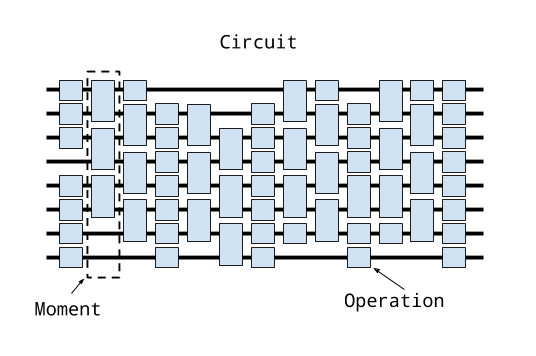
\includegraphics[width=0.8\textwidth]{./chapter2/image/CircuitMomentOperation.png} 
\caption{\label{CircuitMomentOperation} In Cirq a quantum circuit is built thanks to the {\fontfamily{lmtt}\selectfont Circuit} class. A {\fontfamily{lmtt}\selectfont Circuit} object is a collection of moments and each moment is constituted by operation, as gate operations, which act on a subset of qubits. Image from: https://cirq.readthedocs.io/en/stable/circuits.html.}
\end{figure}

\begin{figure}[h!]
\begin{lstlisting}[language=Python]%[language=Python, caption=Python example]

import cirq
import numpy as np
from math import pi
import matplotlib.pyplot as plt
#select the number of qubit and define LineQubits structure
n = 3 
qubits = cirq.LineQubit.range(n)
#create the circuit
def circuit():      
    circuit = cirq.Circuit()            
    circuit.append(cirq.H(qubits[0]))
    for i in range(n-1):    
        circuit.append(cirq.CNOT(qubits[i],qubits[i+1]))    
    #measurement
    circuit.append(cirq.measure(*qubits, key='x'))          
    print(circuit)        
    return circuit
#select the simulator  and execute the circuit
def simulation(circuit):           
    simulator = cirq.Simulator()
    results = simulator.run(circuit, repetitions=100)
    counts = cirq.plot_state_histogram(results)
#main function
def main ():    
    simulation(circuit())        
if __name__ == '__main__':
    main()
\end{lstlisting}
\caption{\label{GHZ_BuildCircuit} Python code for building the quantum circuit for creating a GHZ state of $n=3$ qubits. In the Python function 'circuit' the quantum circuit is built, while in the function 'simulation' the circuit is executed in the desired simulator. The results of the execution are shown in Figure \ref{DataResults_Cirq} on the left. }
\end{figure}

\subsubsection{Parameterized circuits}
The Cirq platform provides useful features for working with parameterized circuits. Cirq allows gates with parameters to have {\fontfamily{lmtt}\selectfont Symbols}, which can be resolved by a {\fontfamily{lmtt}\selectfont ParamResolver} with a given set of values, rather than having to create a new quantum circuit for every new set of variables,  in fact we only have to change the value of the `ParamResolver` to change the circuit. An example of a parameterized circuit is shown in Figure \ref{Cirq_ParameterizedCircuit}.

\begin{figure}[h!]
\begin{lstlisting}[language=Python]%[language=Python, caption=Python example]

import cirq
import numpy as np
from math import pi
import sympy
#define LineQubits structure
qubits = cirq.LineQubit.range(1)
#create the circuit
circuit = cirq.Circuit()
# add a gate with a symbol which can take any value
gate = cirq.X**sympy.Symbol('s')
circuit.append(gate(qubits[0]))
circuit.append(cirq.measure(qubits[0], key="z"))
# get a param resolver
resolver = cirq.ParamResolver({'s': np.pi / 4.0})
# run the resolved circuit using the param resolver
simulator = cirq.Simulator()
results = simulator.run(circuit, resolver, repetitions=100)
counts = cirq.plot_state_histogram(results)
\end{lstlisting}
\caption{\label{Cirq_ParameterizedCircuit} Python code for building a parameterized circuit for $n=1$ qubit in Cirq software. The results of the execution are shown in Figure \ref{DataResults_Cirq} on the right.}
\end{figure}

\subsubsection{Running quantum circuits and simulators}

In Cirq software 'running' a quantum circuit has the same meaning described yet in the section of Qiskit software, so we assume that this concept is already clear. So far, Cirq is not connected to any real device, but according to statements from Google, quantum computer will be available over the cloud in the near future, using Cirq as an interface. Indeed, Cirq already provides details on these devices as for example the architecture of the 22-qubit FoxTail computer or the 72-qubit Bristlecone computer. Althought the cloud service is still unavailable to general users, Cirq provides built in Python simulators for testing small circuits. The two main types of simulations that Cirq supports are pure state and mixed state. The simulators available are:

\begin{itemize}
	\item {\fontfamily{lmtt}\selectfont Simulator}: works for generic gates implementing their unitary matrix. There are two types of methods that simulator supports, the 'run methods' and the 'simulate methods'. The 'run methods' ('run 	and 'run$\_$sweep') 	emulate a run on a quantum computer hardware and only return measurement results without giving access to the wave function. The output is returned as a `Counter` object (Python built-in class) that displays 	key-value pairs corresponding to the output and number of times that output was recorded.  The 'simulate methods' (`simulate`, `simulate$\_$sweep`, and `simulate$\_$moment$\_$steps`) can be used for full access to the 	wave function at the end of the simulation of the circuit. Once the circuit has been simulated, the result is stored and this output supports several useful features as Dirac notation of the state, access to the wave function or the computation of the (reduced) density matrix of the system.
	
	\item {\fontfamily{lmtt}\selectfont google.XmonSimulator}: is specialized for the native gate set of Google’s Xmon hardware. This simulator supports the same method as {\fontfamily{lmtt}\selectfont Simulator} for doing different types of simulations. The only difference is that each gate used, or the map of the circuit, must be adapted for Xmon devices.
	
	\item {\fontfamily{lmtt}\selectfont DensityMatrixSimulator}: supports involving mixed states simulation. In fact, it is a simulator for density matrices and noisy quantum circuits. This simulator supports the same methods of {\fontfamily{lmtt}		\selectfont Simulator} for 	different types of simulation.
\end{itemize}
\noindent
For simulation of a simple quantum algorithm, any quantum computer simulator is essentially equivalent. However, the simulator chosen can become significant when larger numbers of qubits and gates are used in a quantum circuit.
The maximum number of qubits that can be simulated depends on memory of the user’s computer, in fact a large RAM implies larger circuits.
The simulators of Cirq are good utilities but Qiskit ones have a high-performance \cite{SoftwareComparisonGeneral}  \cite{SoftwareComparisonCirq}.

Currently, Cirq supports modeling noise via \textit{operator sum representations} of noise. It consists on the possibility to add in the circuit common channels as Depolarizing channel,  Bit flip channel, Phase flip channel or Amplitude Damping channel. These channels are added in the circuit in the same way as they were gate operations. Unfortunately, at the moment this is the only possibility for modeling noise in Cirq. In fact it is not possible to build a noise model for a given device as in Qiskit software.

In Figure \ref{GHZ_BuildCircuit} or in \ref{Cirq_ParameterizedCircuit}, the {\fontfamily{lmtt}\selectfont Simulator} class is used for doing noiseless simulations. For each circuit, the histogram plots of the data results are shown in \ref{DataResults_Cirq}. 
 
 \begin{figure}
 \begin{minipage}[c]{0.5\linewidth}
\hspace{1cm}
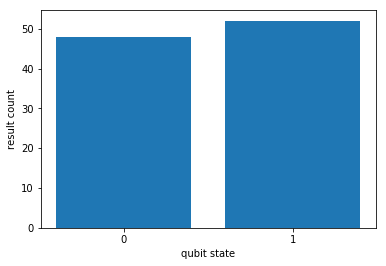
\includegraphics[width=0.8\textwidth]{./chapter2/image/Cirq_GHZ_Histogram.png} 
\end{minipage}
\hspace{-1cm}
% \begin{large} $\Rightarrow$ \end{large}
\begin{minipage}[]{0.5\linewidth}
\centering 
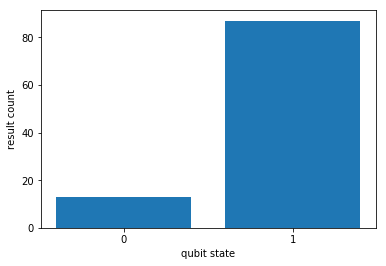
\includegraphics[width=0.8\textwidth]{./chapter2/image/Cirq_ParameterizedCircuit.png} 
\end{minipage}
\caption{\label{DataResults_Cirq} Left: histogram plot of data results of the GHZ quantum circuit of Figure \ref{GHZ_BuildCircuit}. Right: histogram plot of data results of the parameterized circuit of Figure \ref{Cirq_ParameterizedCircuit}.  }
\end{figure}

%The best current methods for classically simulating quantum circuits peak somewhere around 50 qubits due to memory limitations. For a fixed number of qubits, better simulators can simulate circuits with lower overall runtime and potentially even lower memory usage, which are desirable features for many applications. 





%\subsection{Comparisons}
%
%RISCRIVERE MEGLIO!!!
%Nowadays, the IBM project, Qiskit, is more developed than Cirq software. A wide tutorial for Qiskit software is available online that makes this software more approachable for a beginner user than the second, which makes available only the documentation for the python library. Moreover, a wide community for Qiskit software exists. At the moment, the main difference between the two projects is that Qiskit allows the access to a publicly cloud service for a general user, while Cirq provides only simulators as yet, because of a private access to its cloud service. It is expected to change in the future, indeed Google has quantum computers that have been stated to be made available over the cloud soon.
%In general, Cirq is a good tool for writing, manipulating and simulating quantum circuits. In fact, the syntax and organization of the code are very clean as the Python language they are based upon. Cirq allows more flexibility in writing code for a beginner than Qiskit, because its programming language is still in a 'roughly' stage. For example, it allows users to do easily a self-implementation of classe's methods. Consider as an instance the gate implementation. In Cirq it is possible to implement any type of unitary gates and in order to support functionality beyond that basic task, it is necessary to implement several magic methods. In Qiskit it is possible to write a generic gate only combining the operations yet provided. The simulators of Cirq are good utilities but Qiskit ones have a high-performance \cite{SoftwareComparisonGeneral}  \cite{SoftwareComparisonCirq}.
%Probably, the biggest missing feature of Cirq is the ability to simulate noisy quantum circuits, which Qiskit do very well. In fact, in Cirq the modeling of noise is possible only through quantum channels added in the circuit. Instead, in Qiskit it is possible to build a noise model that consists on various types of error on each gate or classical readout errors. In particular, it is possible to build easily a noise model based on parameters of real devices provided by IBM, as we'll see in the next chapter. Instead, one of the best features of Cirq are tools for working with variational quantum algorithms and doing circuit optimization (we just mentioned these arguments because they represents a wide branch of quantum computing and analyze it is beyond the aim of this thesis).
%
%In conclusion, Cirq provides excellent tools for working with circuits for near-term quantum computers but tools provided by Qiskit are more and for the moment they are more developed too. We hope that in the near future, maybe when Google cloud service will be available, the Cirq community will increase and that Cirq library will be more approachable than now.

%For experienced users, Cirq exposes details of the hardware to the programmer to maximize effective utilization of near-term processors.

%In general, we find that Cirq is already a good tool for writing, manipulating, optimizing, compiling, and simulating quantum circuits. For beginners, the learning curve for Cirq is small as the language is written in Python and the syntax/organization of the code is very clean. (We do note that Cirq is written with function annotations in Python which in several cases can be rather verbose.) For experienced users, Cirq exposes details of the hardware to the programmer to maximize effective utilization of near-term processors.
%
%We expect the platform to keep improving as quantum hardware and other simulators are made available. We find the tools for working with variational quantum algorithms, including local simulators as opposed to cloud-based simulators, to be one of the best features of Cirq. (It should be noted that Forest has emphasis on this feature as well, but currently the functionality is smoother with Cirq in the author’s opinion.) The integration with OpenFermion will likely lead to one of the best tools for quantum simulation algorithms, competing with IBM’s QISKit Aqua library. The simulators of Cirq are both good utilities (though not as high-performance as other simulators such as in QISKit Aer or ProjectQ) and will get better with the ongoing work on noise modeling. Additionally, Finally, we expect the quantum channel and stabilizer code features of Cirq to be interesting and useful once they are released.
%
%As mentioned, probably the biggest missing feature of Cirq is the ability to simulate noisy quantum circuits, which Forest and QISKit do very well. (We expect this feature to be released in future versions.) As was seen in the quantum teleportation algorithm, the ability to implement classical operations in circuits, a feature emphasized by the Forest platform, is entirely missing in Cirq. Additionally, the documentation, tutorials, and library support of Cirq are much more sparse than Forest, QISKit, the QDK, and even ProjectQ. (Again, the alpha disclaimer is important here.) Currently, users of Cirq will not be able to connect to real quantum computers as they would with Forest, QISKit, or ProjectQ. Once Foxtail and/or Bristlecone are made available over the cloud, however, this will of course change.






